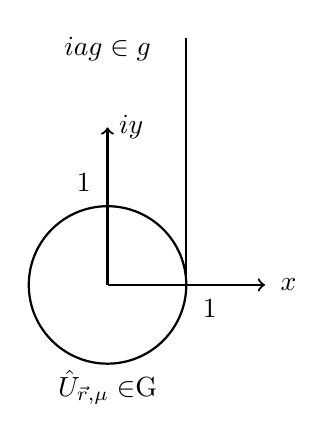
\begin{tikzpicture}
  % Draw the main circle (S^1)
\draw[thick] (0,0) circle(1);

% Parameters
\def\n{5}      % Number of truncation lines (Z5)
\def\r{1}      % Radius of the circle
\def\len{0.2}  % Length of the inward lines

% Draw the 5 truncation lines
\draw[thick] (1, 0) to (1, 3.14);
\draw[thick, ->] (0, 0) to (0, 2);
\draw[thick, ->] (0, 0) to (2, 0);
\node at (0.3,2) {$iy$};
\node at (2.3,0) {$x$};
\node at (-0.3,1.3) {$1$};
\node at (1.3,-0.3) {$1$};
\node at (0, 3) {$iag\in\mathfrak{g}$};
\node at (0, -1.3) {$\hat{U}_{\vec{r}, \mu}\in$G};
 
  
\end{tikzpicture}
